\documentclass[a4paper,12pt]{article}
\usepackage[a4paper,top=1.3cm,bottom=2cm,left=1.5cm,right=1.5cm,marginparwidth=0.75cm]{geometry}
\usepackage{cmap}
\usepackage{mathtext}
\usepackage[T2A]{fontenc}
\usepackage[utf8]{inputenc}
\usepackage[english,russian]{babel}
\usepackage{siunitx}
\usepackage{enumitem}
\usepackage{placeins}

\usepackage{graphicx}
\usepackage{subcaption}
\usepackage{amsmath}

\usepackage{wrapfig}
\usepackage{tabularx}
\usepackage{multirow}

\usepackage{hyperref}
\usepackage[rgb]{xcolor}
\hypersetup{colorlinks=true,urlcolor=blue}
\usepackage{siunitx}
\usepackage{amsmath,amsfonts,amssymb,amsthm,mathtools}
\usepackage{mathtools}
\usepackage{icomma}
\mathtoolsset{showonlyrefs=false}
\usepackage{euscript}
\usepackage{mathrsfs}
\DeclareMathOperator{\sgn}{\mathop{sgn}}
\newcommand*{\hm}[1]{#1\nobreak\discretionary{}
{\hbox{$\mathsurround=0pt #1$}}{}}

%%% Заголовок
\newcommand\labname{Закон Кюри-Вейсса и обменное взаимодействие в ферромагнетиках}
\newcommand\labnumber{6.9.1}


\author{Макаров Лев Евгеньевич}
\title{Лабораторная работа №\labnumber

\labname
}

\date{\today}

\makeatletter
\AddEnumerateCounter{\asbuk}{\russian@asbuk@alph}{щ} % section 8.1
\makeatother

\begin{document}


\begin{titlepage}
	\begin{center}
		{\large МОСКОВСКИЙ ФИЗИКО-ТЕХНИЧЕСКИЙ ИНСТИТУТ (НАЦИОНАЛЬНЫЙ ИССЛЕДОВАТЕЛЬСКИЙ УНИВЕРСИТЕТ)}
	\end{center}
	\begin{center}
		{\large Физтех-школа фотоники, электроники и молекулярной физики}
	\end{center}
	
	
	\vspace{4.5cm}
	{\huge
		\begin{center}
			{\bf Отчёт о выполнении лабораторной работы \labnumber}\\
			\labname
		\end{center}
	}
	\vspace{2cm}
	\begin{flushright}
		{\LARGE Автор:\\ Макаров Лев Евгеньевич \\
			\vspace{0.2cm}
			Б04-306}
	\end{flushright}
	\vspace{8cm}
	\begin{center}
		Долгопрудный 2026
	\end{center}
\end{titlepage}

\section{Введение}


\textbf{Цель работы:} 
\begin{enumerate}
	\item Исследовать зависимость изменения частоты колебаний LC-генератора от температуры вводимого в катушку образца $\text{Gd}^{3+}$
    \item Экстраполируя эту зависимость определить точку Кюри для образца
    \item Определить величину обменного интеграла для этого образца
\end{enumerate}

\textbf{В работе используются:} LC-генератор с катушкой самоиндукции, ферромагнитный образец (гадолиний), термопара, термостат, цифровой частотомер, измерительный милливольтметр.

\section{Теоретические сведения}

Намагниченность вещества $I$ связана с внешним магнитным полем $H$:

\begin{equation}\label{eq:1}
    I = \varkappa H
\end{equation}


где $\varkappa$ - магнитная восприимчивость.


Магнитный момент электрона $\boldsymbol{\mu}$ во внешнем поле будет направлен либо по, либо против поля, поэтому в магнитном поле возникнут энергии


\begin{equation*}
    E_{\pm} = \pm\mu B
\end{equation*}


В состоянии $E_-$ магнитный момент параллелен полю. Отношения числа частиц на этих уровнях


\begin{equation*}   
    \dfrac{N_+}{N_-} = \exp\left(- \dfrac{2\mu B}{k_{\text{Б}}T} \right) \approx 1 - \dfrac{2\mu B}{k_{\text{Б}}T}
\end{equation*}

здесь приближение справедливо, так как даже для $B = 10^5~\text{Гс}$ при $T = 300~\text{К}$ будет справедливо $2\mu B/k_{\text{Б}}T \approx 0.05$, а значит, мы можем считать $\mu B \ll k_{\text{Б}}T$. Соответственно, намагниченность определяется разностью чисел электронов на двух уровнях


\begin{equation*}
    \Delta N = N_- - N_+ \approx N \dfrac{\mu B}{k_{\text{Б}}T}
\end{equation*}

где $N = N_- + N_+$ - количество неспаренных электронов в единице объёма. Отсюда, учитывая $I = \mu \Delta N$ и $H \approx B$, и из \eqref{eq:1} получаем

\begin{equation}\label{eq:2}
    \varkappa = \dfrac{I}{H} = N\dfrac{\mu^2}{k_{\text{Б}}T}
\end{equation}

Для атома с более чем одним электроном и суммарным спином $S$, эта формула обобщается как


\begin{equation*}
    \varkappa = \dfrac{Ng^2 \mu_{\text{Б}}^2S(S+1)}{3k_{\text{Б}}T}
\end{equation*}


где $g$ - фактор Ланде.\\


В ферромагнетиках для описание взаимодействия соседних электронов вводится эффективное (или обменное) поле $H_{\text{эфф}}$, величина которого пропорциональна намагниченности:

\begin{equation*}
    H_{\text{эфф}} = \lambda I
\end{equation*}

где $\lambda$ - некоторая константа. С учётом этого поля формула \eqref{eq:2} преобразуется:

\begin{equation*}
    \varkappa = \dfrac{I}{H} = N\dfrac{g^2 \mu_{\text{Б}}^2 S(S+1)}{3k_{\text{Б}}(T-\Theta)}
\end{equation*}

где 
\begin{equation*}
    \Theta = N \dfrac{g^2 \mu_{\text{Б}}^2 S(S+1)}{3k_{\text{Б}}}\lambda
\end{equation*}

- параметр с размерностью температуры. В итоге получили соотношение


\begin{equation}\label{eq:3}
    \varkappa \propto \dfrac{1}{T - \Theta}
\end{equation}


называемое \textit{законом Кюри-Вейсса}. Температура $\Theta$ называется парамагнитной точкой Кюри, при стремлении температуры к ней восприимчивость неограниченно возрастает из-за того, что тепловое движение всё меньше препятствует магнитным моментам ориентироваться в одном направлении. Это не то же самое, что точка Кюри $T_\text{C}$, которая определяется как температура фазового перехода из парамагнитного в ферромагнитное состояние. Как правило, $\Theta > T_\text{С}$.


Теперь выясним связь обменного интеграла с $\Theta$. Исходя из наличия эффективного поля $H_{\text{эфф}}$, получаем, что энергия, которую необходимо затратить на то, чтобы перевернуть один спин, может быть получена как 


\begin{equation}\label{eq:4}
    U_{\text{пер}} = 2\mu H_{\text{эфф}} = 2 \mu \cdot \lambda I = 2\mu \dfrac{\lambda \mu}{V}
\end{equation}


где $V$ - объём, приходящийся на один атом. В то же время, эта энергия переворота в два раза больше обменной энергии системы, так как можно показать, что энергии систем с параллельными и антипараллельными спинами отличаются знаком. Обменная энергия равна 

\begin{equation*}
    U_{\text{обм}} = -2J \mathbf{S}_i \mathbf{S}_j
\end{equation*}

где $J$ - обменный интеграл, $\mathbf{S}_i \mathbf{S}_j$ скалярное произведение векторов спинов, поэтому в итоге

\begin{equation*}
    U_{\text{пер}} = 2 (2JnS^2)
\end{equation*}

где $S$ - среднее значение $\mathbf{S}$ вдоль направления намагниченности, $n$ - число соседей. Таким образом, с учётом \eqref{eq:4} и $\mu = gS\mu_\text{Б}$, получаем

\begin{equation*}
    \lambda = \dfrac{2nJV}{g^2\mu^2_\text{Б}}
\end{equation*}

Учитывая, что $V = 1/N$, где $N$ - концентрация атомов, то, с учётом определения $\Theta$ получим окончательно

\begin{equation}\label{eq:5}
    J = \dfrac{3k_\text{Б}\Theta}{2nS(S+1)}
\end{equation}


\section{Экспериментальная установка}

Экспериментальная установка для измерения восприимчивости магнетиков приведена на рис. \ref{pic:ustan}.  Ферромагнитный образец 1 располагается внутри пустотелой катушки 2, которая является индуктивностью колебательного контура, входящего в состав LC-генератора. Генератор собран на полевом транзисторе и смонтирован в виде отдельного блока. Частота колебаний генератора высвечивается на цифровом табло блока. Катушка самоиндукции помещена в термостат, представляющий собой массивный медный цилиндр 3, расположенный в пенопластовом корпусе 4. Исследуемый ферромагнетик (гадолиний) является проводником электрического тока, а рабочая частота генератора довольно высока - порядка сотен килогерц. Поэтому для того, чтобы в образце не возникали токи Фуко, маскирующие изучаемый эффект, он изготовлен из мелких гранул размером менее 0,1 мм. Образец помещен в тефлоновую капсулу. С помощью штока 5 капсулу можно перемещать вдоль оси катушки самоиндукции. Когда шток опущен, образец введен в катушку, а когда поднят - образец из неё вынут.



\begin{figure}[h]
    \begin{center}
        
\includegraphics[width = 0.45\textwidth]{pictures/ustan.png}
        \caption{Схема экспериментальной установки: 1 - капсула с образцом; 2 - катушка самоиндукции; 3 - медный цилиндр; 4 - пенопластовый корпус; 5 - шток; 6 - цанговый зажим; 7 - измерительный сплав термопары; 8 - электронагреватель}
    \label{pic:ustan}
    \end{center}
\end{figure}


Магнитная восприимчивость образца определяется по изменению самоиндукции, происходящему при его введении в катушку. Обозначая через $L$ индуктивность катушки с образцом и через $L_0$ её индуктивность в отсутствии образца, получим:

\begin{equation*}
    L=\mu \frac{4 \pi n^{2} S}{l} ; L_{0}=\frac{4 \pi n^{2} S}{l}
\end{equation*}

Где $\mu$ - магнитная проницаемость образца, $n$ - число витков катушки, $l$ - длина катушки, $S$ - её сечение. Тогда, пренебрегая размагничивающим фактором

\begin{equation*}
    \frac{L-L_{0}}{L_{0}} = \frac{\Delta L}{L_{0}} = \mu - 1 = 4 \pi \varkappa
\end{equation*}

Так как частота колебательного контура определяется как:

\begin{equation*}
    f = \frac{1}{2 \pi \sqrt{LC}}
\end{equation*}

то

\begin{equation*}
    \frac{L - L_0}{L_0} = \frac{f_0^2 - f^2}{f^2} = 4 \pi \varkappa
\end{equation*}

И тогда получаем из соотношения \eqref{eq:3}, что

\begin{equation}\label{eq:6}
    \frac{f^2}{f_0^2 - f^2} \propto T - \Theta
\end{equation}

Пользуясь этим соотношением можно вычислить параметр Кюри, по которому после вычислить обменный интеграл по формуле \eqref{eq:5}.

\clearpage

\section{Результаты измерений и обработка данных}

\subsection*{Калибровка термопары}

Сначала по данным термопары получена зависимость температуры от ЭДС. Аппроксимация квадратичным многочленом:

\begin{equation}\label{eq:thermopair}
    t(\varepsilon) = a_0 + a_1 \varepsilon + a_2 \varepsilon^2
\end{equation}

где $\varepsilon$ измеряется в мкВ, а $t$ --- в $^\circ$C. Для коэффициентов получено

\begin{equation*}
    a_0 = 0.165 \pm 0.055,\quad
    a_1 = (2.552 \pm 0.005)\cdot 10^{-2},\quad
    a_2 = (-5.08 \pm 0.01)\cdot 10^{-7}.
\end{equation*}

Погрешность температуры по правилу распространения погрешностей:

\begin{equation}\label{eq:sigma_t}
    \sigma_t = \sqrt{ \sigma_{a_0}^2 + \varepsilon^2 \sigma_{a_1}^2 + \varepsilon^4 \sigma_{a_2}^2 + \left(a_1 + 2 \varepsilon a_2 \right)^2 \sigma_\varepsilon^2 }.
\end{equation}

Результат аппроксимации показан на рис. \ref{pic:thermopair_approximation}.

\begin{figure}[h]
    \begin{center}
        
\includegraphics[width=0.7\textwidth]{pictures/thermopair_approximation.pdf}
        \caption{Аппроксимация температурной характеристики термопары}
        \label{pic:thermopair_approximation}
    \end{center}
\end{figure}

\subsection*{Температурные зависимости частот}

Для измерений учитывалась поправка нуля термопары $V_0 = 0{,}11$ мВ. Температура в кельвинах вычислялась по формулам

\begin{equation*}
    t = t(\varepsilon) + t_0,\quad T = t + T_0,
\end{equation*}

где $t_0 = 26^\circ$C --- комнатная температура, $T_0 = 273{,}15$ K. Для оценки погрешности также использовалась приближенная формула

\begin{equation}\label{eq:sigma_T_approx}
    \sigma_T = \sigma_t = |t - t_0| \sqrt{\left(\frac{\sigma_V}{V}\right)^2 + \left(\frac{\sigma_k}{k}\right)^2}.
\end{equation}

Зависимости $f(T)$ и $f_0(T)$ представлены на рис. \ref{pic:frequencies_temperature}.

\begin{figure}[h]
    \begin{center}
        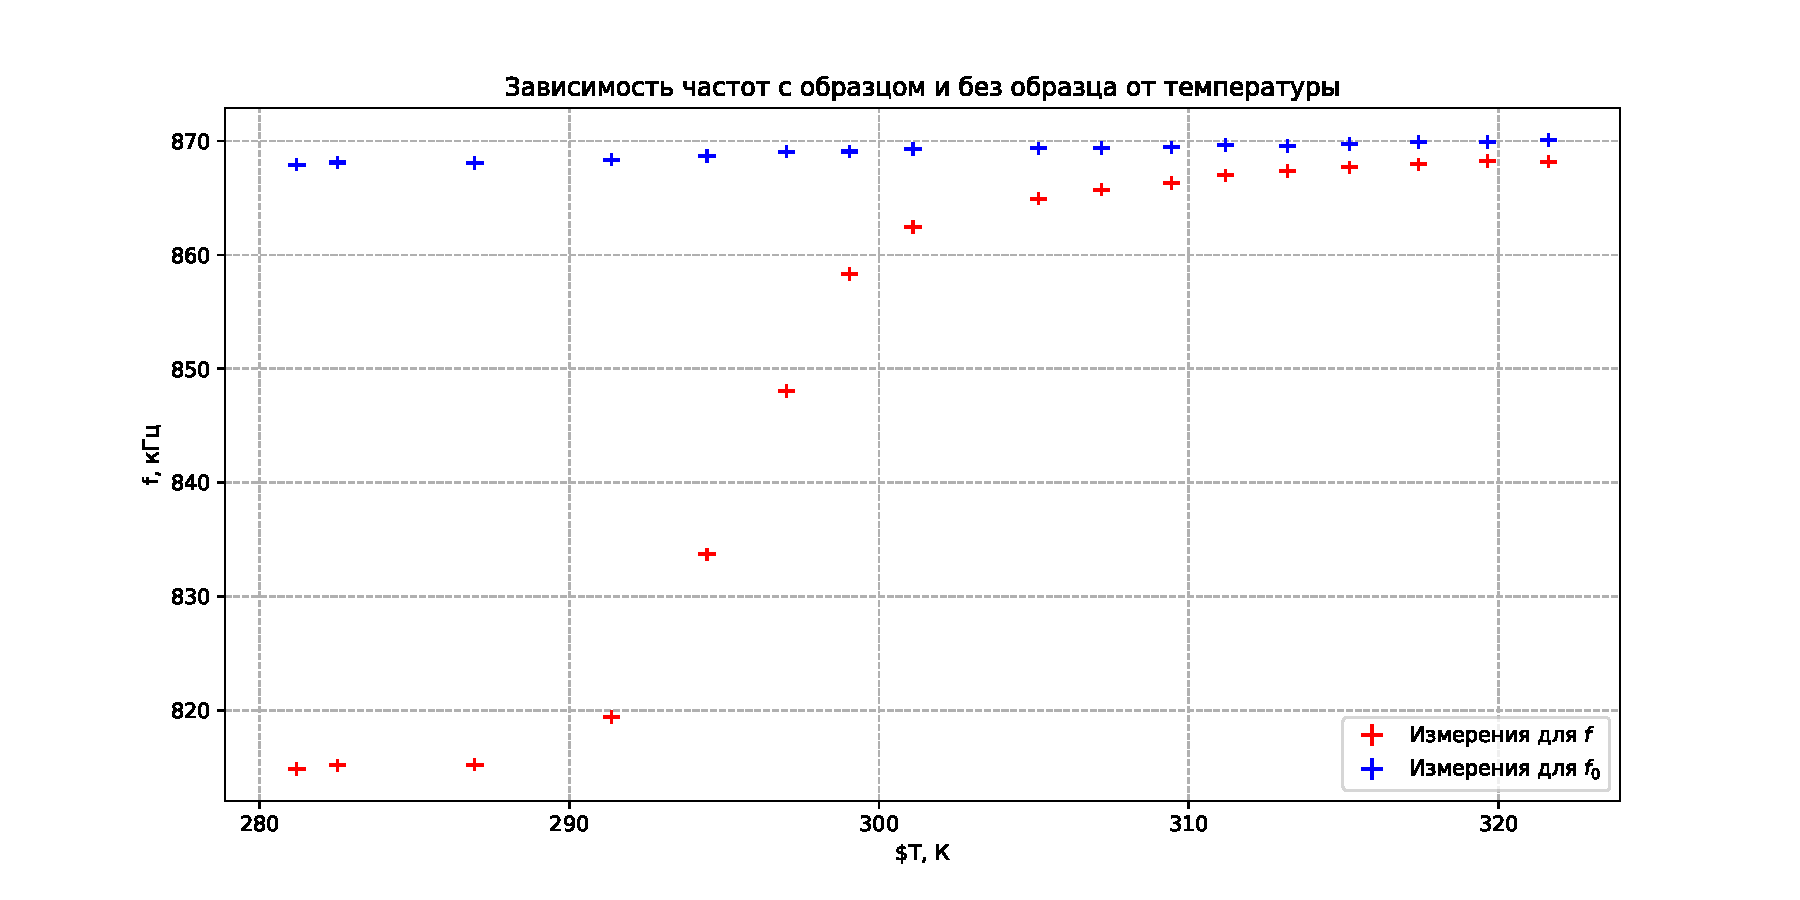
\includegraphics[width=0.75\textwidth]{pictures/frequencies_temperature.pdf}
        \caption{Зависимость частот с образцом и без образца от температуры}
        \label{pic:frequencies_temperature}
    \end{center}
\end{figure}

\subsection*{Определение параметра Кюри}

Для дальнейшей обработки вводим величину

\begin{equation}\label{eq:K}
    K = \frac{f^2}{f_0^2 - f^2}.
\end{equation}

Ее погрешность равна

\begin{equation}\label{eq:sigma_K}
    \sigma_K = \sigma_f \frac{2 f f_0}{\left( f^2 - f_0^2 \right)^2} \sqrt{f^2 + f_0^2}.
\end{equation}

Для линейной области $T > 297$ K (две выбросные точки исключались) аппроксимация дала

\begin{equation*}
    K = kT + b,\quad k = 10{,}55 \pm 0{,}25,\quad b = -3118 \pm 2.
\end{equation*}

Точка Кюри:

\begin{equation}\label{eq:theta}
    \Theta = -\frac{b}{k} = (295 \pm 7)\ \text{K}.
\end{equation}

График и линейная аппроксимация приведены на рис. \ref{pic:kyuri}.

\begin{figure}[h]
    \begin{center}
        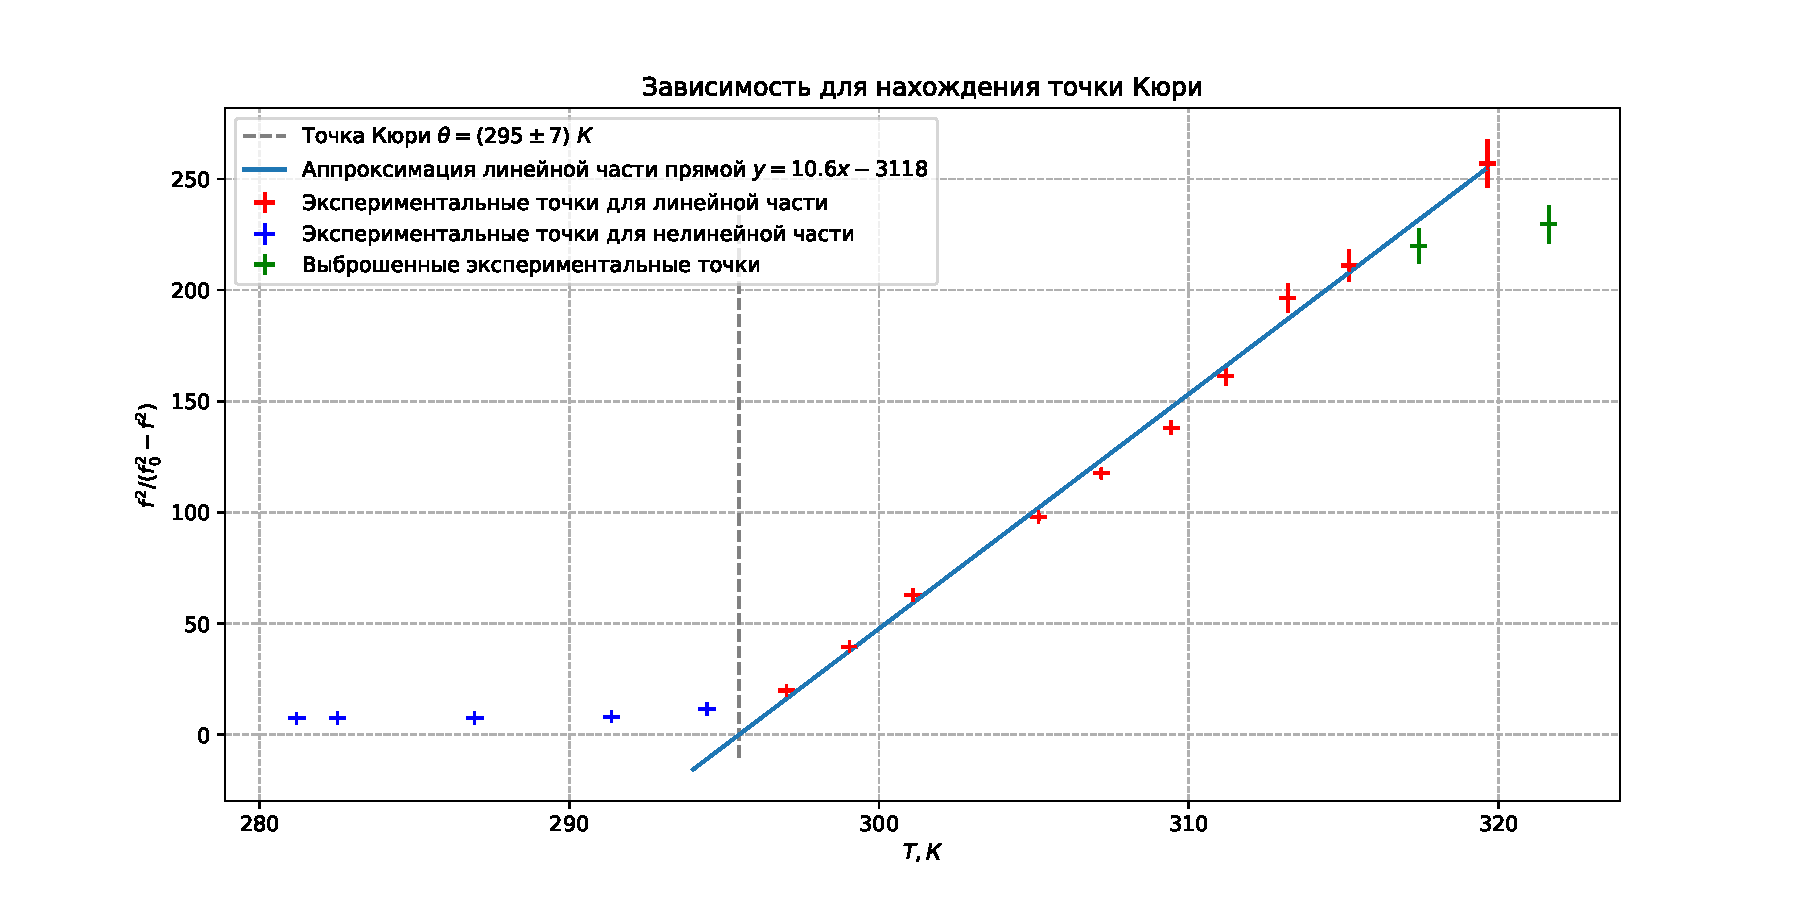
\includegraphics[width=0.75\textwidth]{pictures/kyuri.pdf}
        \caption{Зависимость $K(T)$ и определение точки Кюри}
        \label{pic:kyuri}
    \end{center}
\end{figure}

\subsection*{Обменный интеграл}

Обменный интеграл рассчитывается по формуле

\begin{equation}\label{eq:J}
    J = \dfrac{3k_\text{Б}\Theta}{2nS(S+1)},
\end{equation}

где для гадолиния $n = 12$, $S = 7/2$. Получаем

\begin{equation*}
    J = (3{,}24 \pm 0{,}08)\cdot 10^{-23}\ \text{Дж}
    = (2{,}35 \pm 0{,}05)\ \text{K}
    = (202 \pm 5)\ \text{мкэВ}.
\end{equation*}

\subsection*{Магнитная восприимчивость}

Восприимчивость оценивалась по выражению

\begin{equation}\label{eq:kappa}
    \varkappa = \frac{1}{4 \pi} \frac{f_0^2 - f^2}{f^2} = \frac{1}{4 \pi K}.
\end{equation}

Погрешность:

\begin{equation}\label{eq:sigma_kappa}
    \sigma_\varkappa = \frac{\sigma_K}{4 \pi K^2} = \varkappa \frac{\sigma_K}{K}.
\end{equation}

График зависимости $\varkappa(T)$ приведен на рис. \ref{pic:kappa_graph}.

\begin{figure}[h]
    \begin{center}
        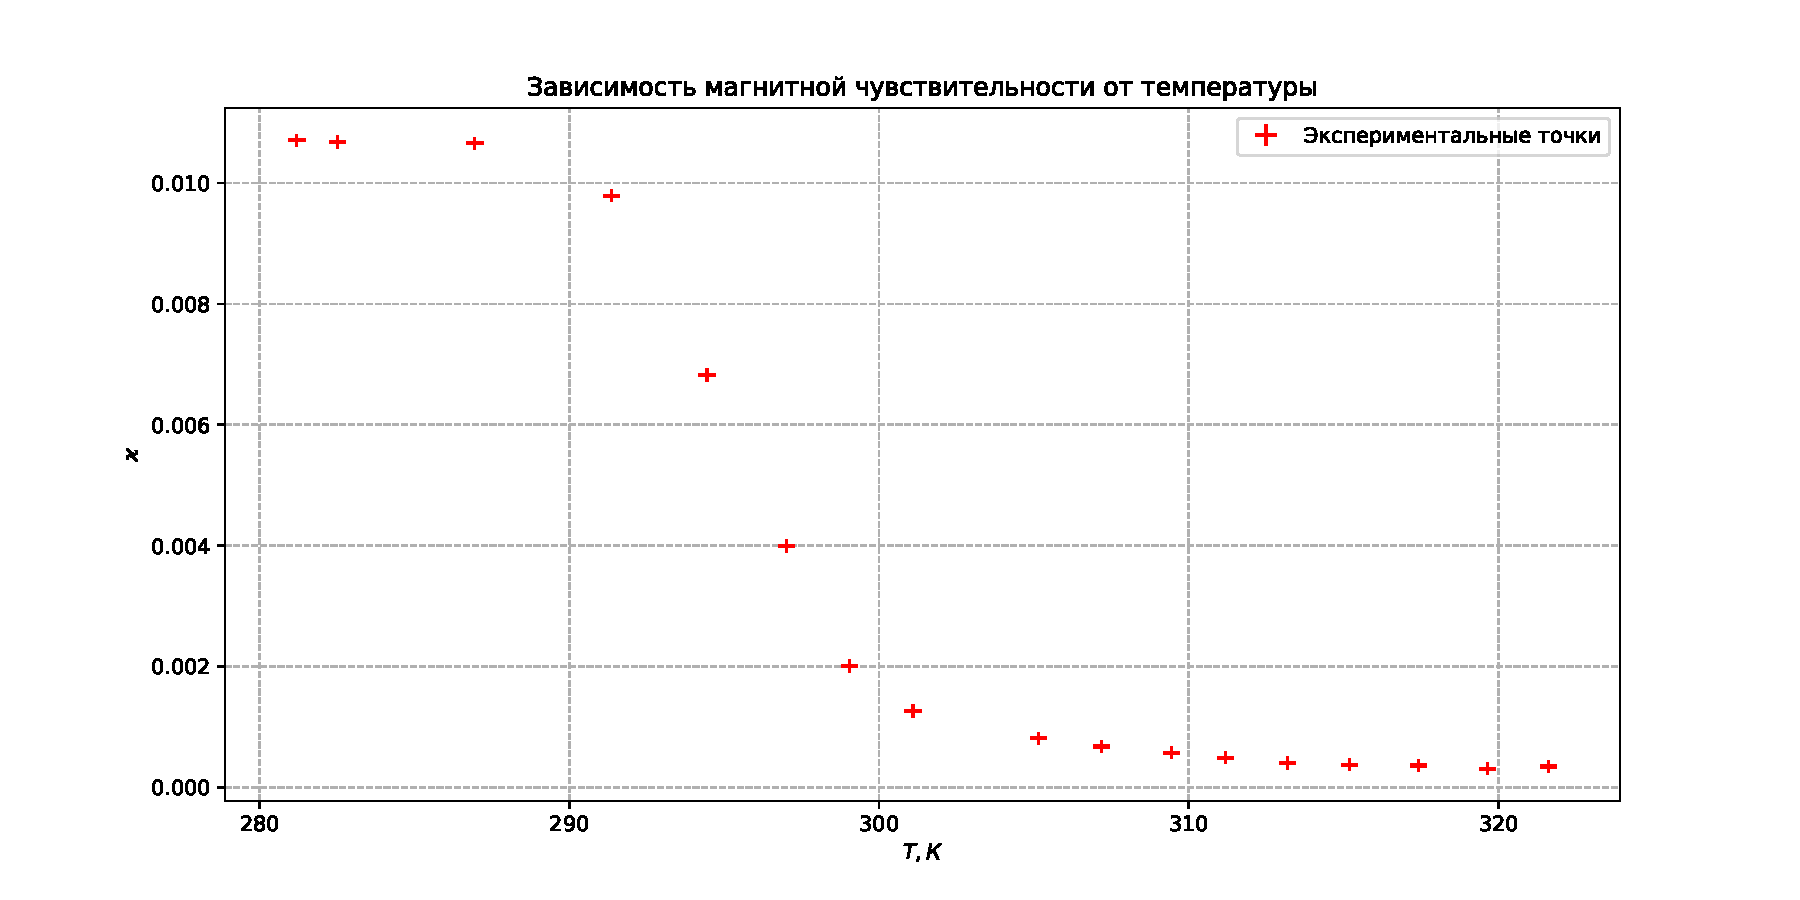
\includegraphics[width=0.75\textwidth]{pictures/kappa_graph.pdf}
        \caption{Зависимость магнитной восприимчивости от температуры}
        \label{pic:kappa_graph}
    \end{center}
\end{figure}

\subsection*{Проверка аппроксимации}

Критерий согласия:

\begin{equation}\label{eq:chi2}
    \chi^2 = \sum \frac{\left( y - \hat{y} \right)^2}{\sigma_y^2 + \sigma_{\hat{y}}^2},
\end{equation}

где $\hat{y} = kx + b$, а

\begin{equation*}
    \sigma_{\hat{y}} = \sqrt{ k^2 \sigma_x^2 + x \sigma_k^2 + \sigma_b^2 }.
\end{equation*}

Для линейной области получено $\chi^2 = 0{,}05$, что указывает на хорошее согласие аппроксимации с данными.

\section{Заключение}

Экспериментально исследована температурная зависимость частоты LC-генератора с образцом гадолиния. По линейной аппроксимации зависимости $K(T)$ получен параметр Кюри $\Theta = (295 \pm 7)$ K. На его основе вычислен обменный интеграл $J = (3{,}24 \pm 0{,}08)\cdot 10^{-23}$ Дж. Наблюдается рост магнитной восприимчивости при приближении к $\Theta$, что соответствует закону Кюри-Вейсса.

\end{document}
